\chapter{Analysis of Sparse Triangular Solve} 
%\section{Analysis of the Forward/Backward Substitution} 
\label{sec:sds}

% \mycomment{OR: Werden die Daten analysiert oder ihr Transfer? MW: der Transfer
% natürlich :)}
In this section, we analyze the data transfer between the different cache levels
and the FLOPs performed during  the
sparse triangular solve phase.
%\sout{\OR the forward/backward substitution.}
% \mycomment{OR: Fehlender Bezug durch ``which''. MW: OK}
The results are used as input for our performance model 
to be
established in the next section.
%
Therefore, we inspect the different instantiations of the loops resulting from
Algorithm~\ref{alg:algo:fw} and~\ref{alg:algo:bw}.
% \mycomment{``Hereby'' heisst ``hierdurch'', nicht ``hierbei''}
Here, we only consider the innermost loops and do not 
distinguish between updates of~\vr{} or temporary arrays~\vtemp{}.

All entries %\sout{coefficients} 
of the $L$ matrix
% \mycomment{OR: Bezeichnung ``coefficients'' hier gut? MW: entries? OR: OK.}
are stored as double-precision floating point
numbers in \vlnz{}, consuming $8$\,B (byte) each. 
Elements of the \vxlnz{} (column start indices in \vlnz{}) and \vxindx{} (start
indices of row indices for each panel) arrays are stored as $8$\,B integers,
whereas for the entries of \vindx{} (row indices for each panel) $4$\,B integers
are used.

\section{Data transfers and FLOPs without unrolling}
\label{sec:pm:dt}
\label{sec:pm:dt:wou}

% \begin{figure}[t]
%   \centering
%  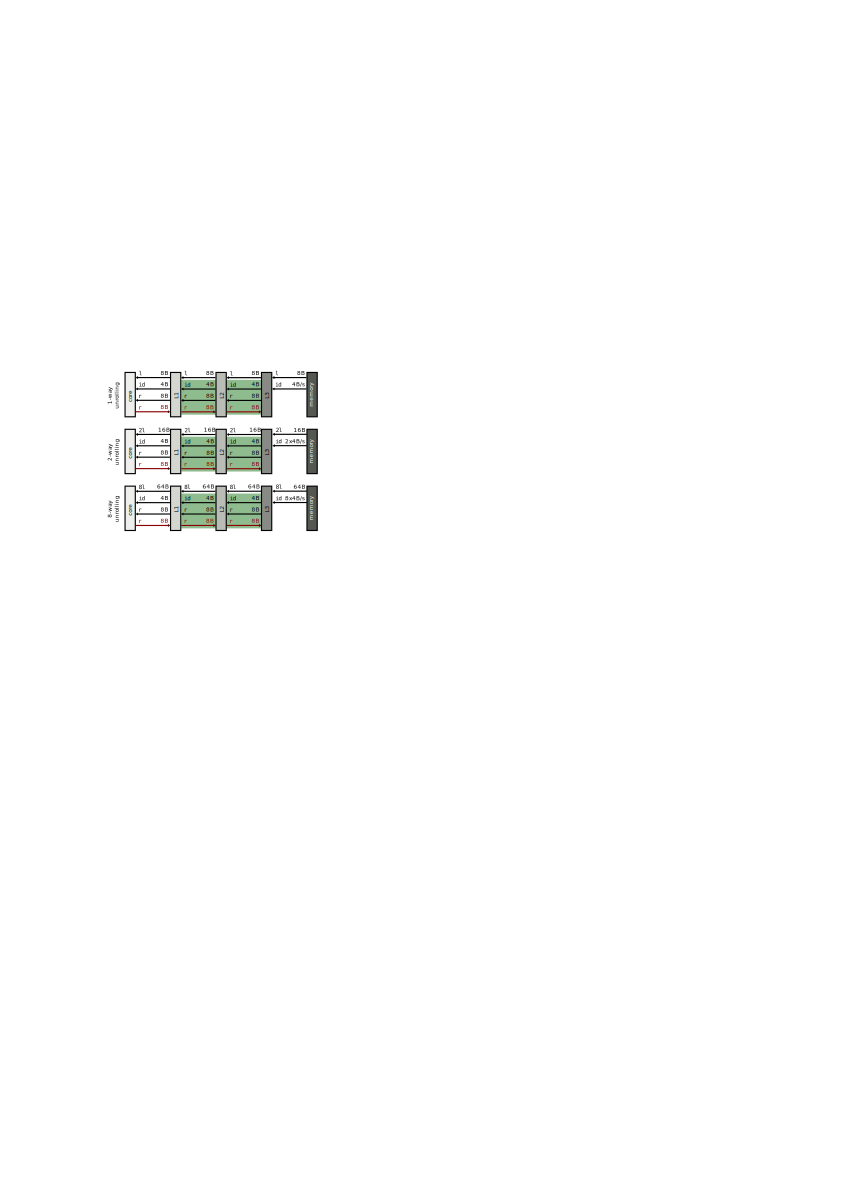
\includegraphics[width=0.43\textwidth,clip=true]{images/ecm-datatransfers}
%   \caption{Data transfers for one iteration of the forward
%     (including red text and arrows) and backward (without red text and arrows)
%     substitution when $1$-, $2$-, or $8$-way column unrolling is applied.
%     Thereby $1$, $2$, or $8$ nonzero elements of \vlnz{} are processed,
%     respectively.
% %    Loading of \vindx{} from memory (blue boxes) is only included in the model 
% %    if the panel size $s \le 8$.
% % From which cache level \vr{} is reused (green boxes) depends on the size of the
% % active part. If the active part is large it must be reloaded from
% % L3 cache. With decreasing size it can fit into L2 or even L1 cache.
% % This holds also true for \vindx{}, but additionally depends on the panel size.
%   }
%   \label{fig:ecm:data}
% \end{figure}
% 

\begin{figure}[t]
  \centering%
%  \includegraphics[width=0.3\textwidth,clip=true]{images/ecm-datatransfers-1}
%  \includegraphics[width=0.3\textwidth,clip=true]{images/ecm-datatransfers-2}
%  \includegraphics[width=0.3\textwidth,clip=true]{images/ecm-datatransfers-8}
  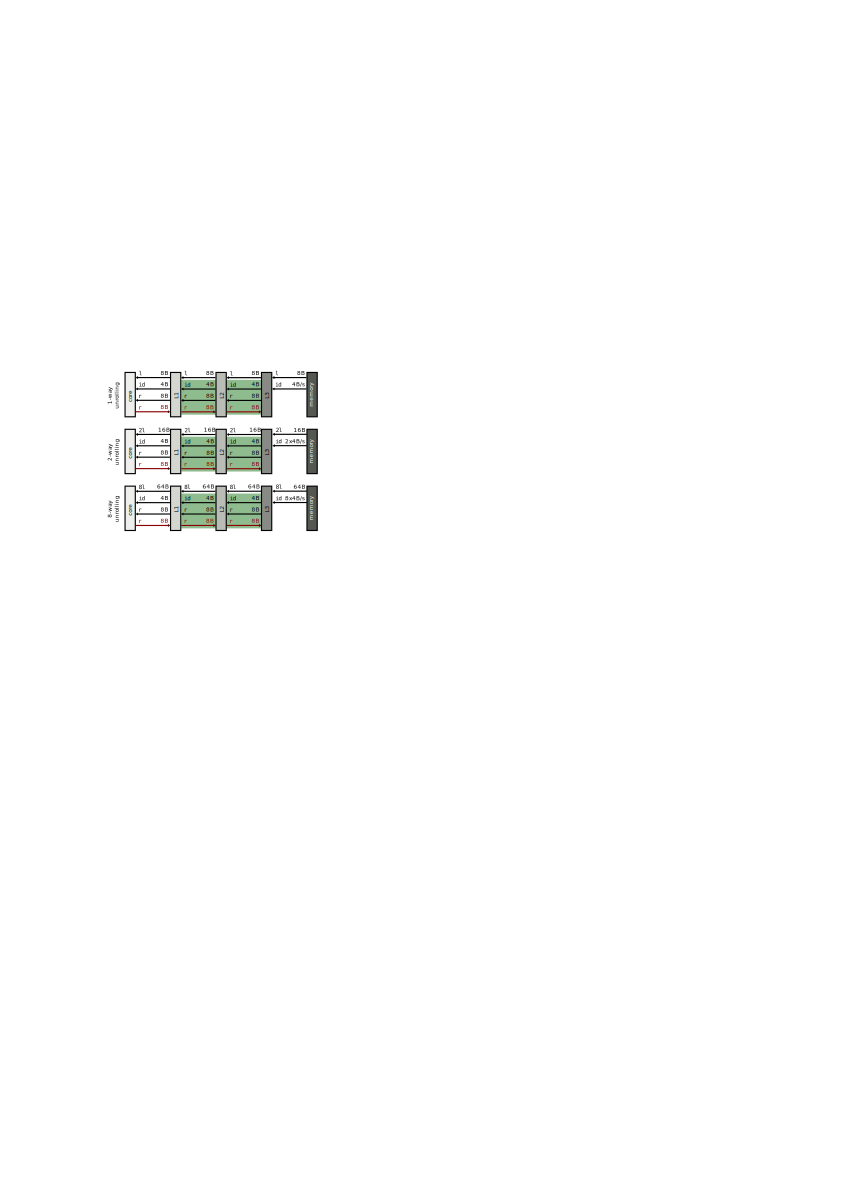
\includegraphics[width=0.75\linewidth,clip=true]{images/ecm-datatransfers}
  \caption{Data transfers for one iteration of the forward
    (including red text and arrows) and backward (without red text and arrows)
    substitution when $1$-, $2$-, or $8$-way column unrolling is applied 
    for a panel with panel size $s$.
    Thereby $1$, $2$, or $8$ nonzero elements of \vlnz{} are processed,
    respectively.
%    Loading of \vindx{} from memory (blue boxes) is only included in the model 
%    if the panel size $s \le 8$.
% From which cache level \vr{} is reused (green boxes) depends on the size of the
% active part. If the active part is large it must be reloaded from
% L3 cache. With decreasing size it can fit into L2 or even L1 cache.
% This holds also true for \vindx{}, but additionally depends on the panel size.
  }
  \label{fig:ecm:data}
\end{figure}

In the most simple case no unrolling is applied and the innermost loop of
forward substitution from Algorithm~\ref{alg:algo:fw} looks like
% \mycomment{OR: sollte der Alg.~\ref{alg:algo:fw} nicht
% eine Float-Umgebung bekommen? MW: algorithm ist doch eine float-Umgebung.
% OR: Habe mich vertan.
% }
%
\begin{algorithmic}[1]
  \setcounter{ALG@line}{22}
  \For{k = \nxlnz[j] + offset; k < \nxlnz[j+1]; ++k}
      \State row = \nindx[i++]
      \State \nr[row] -= \nr[j] \nlnz[k]
  \EndFor
\end{algorithmic}%
%\vspace{-\baselineskip}
\noindent%
%
As the loops from lines $6$--$9$ and $10$--$13$ are in principle identical to
the loops in lines $23$--$26$, we only discuss the latter.
%
During each iteration one nonzero is processed, two FLOPs are performed,
namely, a multiplication and an addition, and the following elements get
loaded and stored, loaded: \vindx{} ($4$~\,B), \vr{} ($8$~\,B), \vlnz{}
($8$~\,B); stored: \vr{} ($8$~\,B).

How much data are transferred inside the cache hierarchy depends on the size of
the caches, their replacement strategies, the size of \vr{}, the average panel
size, as well as the structure of the panels, i.\,e.,\ which part of \vr{} is
accessed.
Here we assume \vr{} is small enough to be kept at least in last level cache
(LLC) and temporal locality ensures it is not evicted.
%
Row indices in \vindx{} for a panel are loaded from memory for the panel's first
column and then are reused during each iteration over the panel's remaining
columns from the LLC in the worst case.
With panel size $\panelsize=1$, for each element of \vlnz{} one row index is
transferred and no reuse is possible.
In general reuse is only possible, starting with a panel's second column for
panel sizes $\panelsize \ge 2$.
%
Coefficients of \vlnz{} are always streamed in from memory, as they are
used only once and the \vlnz{} array is typically too large to be kept in LLC.
Figure~\ref{fig:ecm:data} visualizes the transfers assuming three cache levels
and \vr{} is cached in LLC.

While iterating over panels and columns, the number of column elements
decreases as $L$ is a lower triangular matrix.
Thereby the number of used elements from \vr{} also decreases, which we call the
active part of \vr{}.
At some point the active part can be completely kept in the L2 or even the L1 cache.
This also holds true for \vindx{}, except when a new panel starts, then
the panel's row indices must first be loaded from memory.
%
%1 The active part of \vr{} can be kept inside a certain cache size $c_s$, when
%1 concurrently also one column of \vlnz{} and the active part of \vindx{} fit into
%1 this cache level.
%1 Let $n_j$ the length of column $j$. 
%1 If $L$ is dense, like for the dense matrix, then if $n_j \le c_s/(8\,\text{B} + 8\,\text{B} +
%1 4\,\text{B})$ holds true all active parts fit into the cache.
%1 %
%1 If instead in the worst case $L$ is sparse so that only one element out of a cache
%1 line from \vr{} is accessed
%1 then $n_j \le c_s/(8\,\text{B} + 64\,\text{B} + 4\,\text{B})$ is required.
%1 %
%1 Note that already when the active part of \vr{} slightly exceeds the determined
%1 limits already partial caching in the same cache level takes place\footnote{If
%1 we
%1 load a vector which exceeds the cache size several times it must be completely
%1 reloaded during each iteration. 
%1 However, if the cache utilizes a least recently used policy and the vector's
%1 size is in the range of the cache size $c_s$ and $c_s + w_s$, where $w_s$
%1 denotes the way size of the cache, then still parts of the vector are held in
%1 the cache and need not to be reloaded.
%1 The way size of a cache is defined as the product of the cache's number of sets
%1 and the cache line size.}.

The innermost loop of the backward substitution from
Algorithm~\ref{alg:algo:bw}, is %looks like 
% The innermost loop from lines $5$--$9$ is the same as the one from lines
% $17$--$20$ of the backward
% substitution from Algorithm~\ref{alg:algo:bw}, which we only discuss the former,
% which looks like 
%
\begin{algorithmic}[1]
\setcounter{ALG@line}{4}
  \For{k = \nxlnz[j] + offset; k < \nxlnz[j+1]; ++k}
    \State row = \nindx[i++]
    \State \nr[j] = \nr[j] - \nr[row] \nlnz[k]
  \EndFor
\end{algorithmic}%
%\vspace{-\baselineskip}
\noindent%
%
As this loop from lines $5$--$8$ is the same as the one from lines $17$--$20$,
all following statements hold true for both. 
%
As with forward substitution one nonzero is processed, two FLOPs are performed,
but only loads occur: \vindx{} ($4$~\,B), \vr{} ($8$~\,B), and \vlnz{} ($8$~\,B).
Note that $j$ is unchanged in the innermost loop, hence $\nr[j]$ always refers
to the same element and is not considered for the data transfer analysis.
%
Figure~\ref{fig:ecm:data} displays the data transfers occurring for one
nonzero update if \vr{} is cached in L3 cache.

\section{Data transfers and FLOPs with unrolling}
\label{sec:pm:dt:wu}

%
As noted in section~\ref{sec:algo} it is beneficial to handle several columns
at once.
%\sout{In PARDISO loops over columns \uwave{are additionally to no unrolling manually $2$- and $8$-times unrolled and used when a panel contains more than one column.}}
For this purpose PARDISO has additionally 2- and 8-way manually unrolled
loops over columns.  These are used when a panel contains more than one column.
With an unrolling factor of two the innermost loop for forward substitution becomes
%
\begin{algorithmic}[1]
  \State nj = nonzero column length
  \For{k = \nxlnz[j] + offset; k < \nxlnz[j+1]; \textcolor{blue}{k += 2}}
      \State row = \nindx[i++]
      \State \nr[row] = \nr[row] - \nr[j] \nlnz[k] \textcolor{blue}{- \nr[j+1] \nlnz[k+nj]}
  \EndFor
\end{algorithmic}%
%\vspace{-\baselineskip}
\noindent%
%
%\sout{\uwave{In contrast to no unrolling per iteration two nonzeros are processed.}}
Instead of processing only one nonzero the 2-way unrolling handles two
nonzeros per iteration.
Hence, four FLOPs are performed and two entries of \vlnz{} are loaded.
Hereby the corresponding element of \vr{} only needs to be loaded once instead of
twice, when processing two elements of \vlnz{}.
All other transfers stay unchanged.
%
In general with a $u$-way unrolling during each iteration, $2 \times u$\,FLOPs
are executed and $u \times 8\,\text{B} + 20\,\text{B}$ are transferred.

Unrolling of the backward substitution loop results in the following code for a
$2$-way unrolling:
%mw2018-06-07: \mycomment{ML: Bin fuer konsistenz: two-way und two-time
%mw2018-06-07: unrolling oder 2-way und 2-time unrolling. MW: OK}
%
\begin{algorithmic}[1]
  \State nj = nonzero column length
  \For{k = \nxlnz[j] + offset; k < \nxlnz[j+1]; \textcolor{blue}{k += 2}}
      \State row = \nindx[i++]
      \State \nr[j]   = \nr[j] - \nlnz[k] \nr[row]
      \State \textcolor{blue}{\nr[j+1]   = \nr[j+1] - \nlnz[k+nj] \nr[row]}
  \EndFor
\end{algorithmic}%
%\vspace{-\baselineskip}
\noindent%
%
Also here four FLOPs per iteration are performed, two entries of \vlnz{} are
loaded and the corresponding element of \vr{} is loaded only once.
%
For a $u$-way unrolling $2 \times u$\,FLOPs and $u \times 12\,\text{B} +
8\,\text{B}$ are loaded.

As already noted, we assume \vr{} and a panel's current row indices from
\vindx{} are at least cached in LLC or higher cache levels.
%
Unrolling, hereby, only saves transfers inside the cache hierarchy.
The bytes transferred between memory and LLC are left unaffected and depend only
on the panel size.
With larger panel sizes in total, fewer
row indices \vindx{} are needed for the
whole matrix.

\section{ECM -- Forward and Backward Substitution}
\label{sec:ecm-fwbw}

\todop{ \\
Algorithm similar to indexed daxpy (Section \ref{sec:ecm-indirect-daxpy}). \\
Detailed description of the algorithm in Chapter \ref{sec:algo}. \\
Analysis of the code including unrolling in Chapter \ref{sec:sds}. \\
\\
Computations here\\
Elements form L are used only once, hence they are always fetched from the memory. We can ignore the tL1..tL3. \\
\\}

Both forward and backward substitution (described in Chapter \ref{sec:algo}) are similar to the indexed daxpy kernel analyzed in Section \ref{sec:ecm-indirect-daxpy}.
The overlapping part of in-core execution is exactly the same as in the indirect daxpy.
Again we take 8 iterations (or 8 rows) as an unit of work, because it fills one cache line. Note that the supernodes in L are stored column-wise, ignoring the sparsity, as described in Chapter \ref{sec:algo}.
We will take into account 1 column for 1-way unroling, 2 columns for 2-way unrolling and 8 columns for 8-way unrolling.
This gives
\begin{eqnarray}
   t^1_\text{ol} & = & \ \ 6\,\cyw \\
   t^2_\text{ol} & = & 12\,\cyw \\
   t^8_\text{ol} & = & 48\,\cyw
\end{eqnarray}

In PARDISO always the most efficient code is used. When a supernode has eight or more columns, the 8-way unrolling is used. 2-way unrolling is used for the remining columns and 1-way unrolling is used only for one column, in case the number of columns is odd.
id is loaded only once per supernode. It could happen in any of the code variants 1-, 2- or 8-way unrolled, depending on the size of the supernode, as shown in Figure \ref{fig:ecm:data}.
We assume id is always loaded from memory in the 1-way unrolled code and for the 2- or 8-way unrolled code it is already present in cache. This allows us to keep the model simple and independent of the nonzero structure of the matrix and its factor L.

In the indexed daxpy r was loaded and stored from/to memory. The right hand side is often assembled just before calling the forward and backward substitution, so it is reasonable to assume that r is already in the cache. We also assume r is small enough to fit the L3 (LLC) cache and as it is used again and again, so it is not evicted.
In case that r was not already present in the cache, it has to be loaded from memory. For reasonably big matrices we can ignore this load from memory, as it happens only once, and assume it is always present in the cache.

There is one difference between the forward and backward substitution in the access pattern to r.
The forward substituion updates different entries in r, the backward substitution always updates the same entry. The updated values in the forward substitution need to be stored in cache after every update (red text and arrows in Figure \ref{fig:ecm:data}), while the only value updated in the backward substituion is kept in register.

Unlike in the daxpy case, the amount of data transfered between adjacent cache levels or L1 and registers is different from what is transfered between L3 and memory. We define the work to be for the forward substitution
\begin{eqnarray}
   W^{\text{fw}-1}_\text{cache} & = & 0\,\Bw \\
   W^{\text{fw}-1}_\text{mem}   & = & 0\,\Bw \\
   W^{\text{fw}-2}_\text{cache} & = & 0\,\Bw \\
   W^{\text{fw}-2}_\text{mem}   & = & 0\,\Bw \\
   W^{\text{fw}-8}_\text{cache} & = & 0\,\Bw \\
   W^{\text{fw}-8}_\text{mem}   & = & 0\,\Bw \\
\end{eqnarray}
and for the backward substitution
\begin{eqnarray}
   W^{\text{bw}-1}_\text{cache} & = & 0\,\Bw \\
   W^{\text{bw}-1}_\text{mem}   & = & 0\,\Bw \\
   W^{\text{bw}-2}_\text{cache} & = & 0\,\Bw \\
   W^{\text{bw}-2}_\text{mem}   & = & 0\,\Bw \\
   W^{\text{bw}-8}_\text{cache} & = & 0\,\Bw \\
   W^{\text{bw}-8}_\text{mem}   & = & 0\,\Bw
\end{eqnarray}
For details please refer to Figure \ref{fig:ecm:data}.

The inputs for the ECM model are summarized in Table \ref{tab:ecm:data}. The values are normalized for 1 column.

\begin{table}[!t]
  \centering
  \begin{tabular}{|l|c|c|c|c|c|c|}
     \hline
      & forward & backward \\
     \hline
      & 1-way & 2-way & 8-way & 1-way & 2-way & 8-way \\
     \hline
     W & 0 & 0 & 0 & 0 & 0 & 0 \\
     \hline
  \end{tabular}
  \caption{\todol{...}}
  \label{tab:ecm:data}
\end{table}
